\documentclass[titlepage, fleqn, a4paper, 12pt, twoside]{article}
\usepackage{geometry}
\usepackage{exsheets} %question and solution environments
\usepackage{amsmath, amssymb, amsthm} %standard AMS packages
\usepackage[utf8]{inputenc}
\usepackage{esint} %integral signs
\usepackage{marginnote} %marginnotes
\usepackage{gensymb} %miscellaneous symbols
\usepackage{commath} %differential symbols
\usepackage{xcolor} %colours
\usepackage{cancel} %cancelling terms
\usepackage[free-standing-units,space-before-unit]{siunitx} %formatting units
	\sisetup
	{
		per-mode=fraction,
		fraction-function=\frac
	}
\usepackage{tikz, pgfplots} %diagrams
	\usetikzlibrary{calc, hobby, patterns, intersections, angles, quotes, spy}
\usepackage{graphicx} %inserting graphics
\usepackage{hyperref} %hyperlinks
\usepackage{datetime} %date and time
\usepackage{enumerate, enumitem} %numbered lists
\usepackage{float} %inserting floats
\usepackage[american voltages]{circuitikz} %circuit diagrams
\usepackage{setspace} %double spacing
\usepackage{microtype} %micro-typography
\usepackage{listings} %formatting code
	\lstset{language=Matlab}
	\lstdefinestyle{standardMatlab}
	{
		belowcaptionskip=1\baselineskip,
		breaklines=true,
		frame=L,
		xleftmargin=\parindent,
		language=C,
		showstringspaces=false,
		basicstyle=\footnotesize\ttfamily,
		keywordstyle=\bfseries\color{green!40!black},
		commentstyle=\itshape\color{purple!40!black},
		identifierstyle=\color{blue},
		stringstyle=\color{orange},
	}
\usepackage{booktabs}
\usepackage{multirow}
\usepackage{todonotes}
\usepackage[noabbrev,capitalize]{cleveref}
\usepackage[section]{placeins}
\usepackage[style=numeric, backend=biber]{biblatex}

% \bibliography{<mybibfile>}% ONLY selects .bib file; syntax for version <= 1.1b
\addbibresource{bibliography.bib}% Syntax for version >= 1.2

\newcommand\numberthis{\addtocounter{equation}{1}\tag{\theequation}} %adds numbers to specific equations in non-numbered list of equations

\DeclareMathAlphabet{\mathcal}{OT1}{pzc}{m}{it}

\theoremstyle{definition}
\newtheorem{example}{Example}
\newtheorem{definition}{Definition}

\theoremstyle{theorem}
\newtheorem{theorem}{Theorem}
\newtheorem{law}{Law}

\makeatletter
\@addtoreset{section}{part} %resets section numbers in new part
\makeatother

\newcommand\blfootnote[1]{%
	\begingroup
	\renewcommand\thefootnote{}\footnote{#1}%
	\addtocounter{footnote}{-1}%
	\endgroup
}

\renewcommand{\marginfont}{\scriptsize \color{blue}}

\renewcommand{\tilde}{\widetilde}

\def\doubleunderline#1{\underline{\underline{#1}}}

\SetupExSheets{solution/print = true} %prints all solutions by default

\DeclareMathOperator{\FT}{\mathcal{F}}
\DeclareMathOperator{\IFT}{\mathcal{F}^{-1}}
\DeclareMathOperator{\LT}{\mathcal{L}}

\DeclareMathOperator{\sinc}{\mathrm{sinc}}
\DeclareMathOperator{\rect}{\mathrm{rect}}

%opening
\title{Wave Transmission}
\author{Aakash Jog}
\date{2016-17}

\begin{document}

\pagenumbering{roman}
\begin{titlepage}
\newgeometry{margin=0cm}
\maketitle
\end{titlepage}
\restoregeometry
%\setlength{\mathindent}{0pt}

\blfootnote
{
	\begin{figure}[H]
		\includegraphics[height = 12pt]{cc.pdf}
		\includegraphics[height = 12pt]{by.pdf}
		\includegraphics[height = 12pt]{nc.pdf}
		\includegraphics[height = 12pt]{sa.pdf}
	\end{figure}
	This work is licensed under the Creative Commons Attribution-NonCommercial-ShareAlike 4.0 International License. To view a copy of this license, visit \url{http://creativecommons.org/licenses/by-nc-sa/4.0/}.
} %CC-BY-NC-SA license

\tableofcontents

\clearpage
\section{Lecturer Information}

\textbf{Prof. Ehud Heyman}\\
~\\
Office: Maabadot 242\\
E-mail: \href{mailto:heyman@tau.ac.il}{heyman@tau.ac.il}\\

\section{Instructor Information}

\textbf{Ram Tuvi}\\
~\\
Office: Tochna 208\\
E-mail: \href{mailto:ramtuvi@post.tau.ac.il}{ramtuvi@post.tau.ac.il}\\

\section{Recommended Reading}

\begin{enumerate}
	\item \fullcite{Orfanidis}
	\item \fullcite{Ramo}
	\item \fullcite{Inan}
	\item \fullcite{Johnk}
	\item \fullcite{Collin}
	\item \fullcite{Pozar}
\end{enumerate}

\clearpage
\pagenumbering{arabic}

\part{}

\section{Lumped and Distributed Circuits}

\begin{definition}[Lumped and distributed circuits]
	A circuit is said to be lumped if the signal generated by the source is unchanged in the time taken for the signal to propagate from the source to the load and back.
	If the signal is harmonic with time period $T$, the circuit is lumped if and only if
	\begin{align*}
		2 L &\ll c T\\
		&\ll \lambda\\
		&\le c \frac{T}{2 M}
	\end{align*}
	where $L$ is the length of the circuit, and $M$ is a constant determined by the requirements.
	\footnote{Typically, $M \ge 8$, i.e. the delay is at most $\SI{22.5}{\degree}$.}\\
	Circuits which are not lumped are called distributed circuits.
	In distributed circuits, the transmission line is also a non-negligible circuit element.
\end{definition}

\clearpage
\part{TEM Transmission Lines}

\section{Modelling a TEM Transmission Line}

\begin{definition}[TEM transmission line]
	A transmission line which allows transverse electromagnetic waves, i.e. electromagnetic waves in which the fields have transverse components only, is called a transverse electromagnetic transmission line or a TEM line.
	Such lines have at least two conductors.
\end{definition}

\begin{definition}
	An infinitesimal section of a transmission line in the $z$ direction can be modelled as in \cref{fig:model_of_infinitesimal_section_of_transmission_line},
	where $C$ is the capacitance per unit length between the wires, $L$ is the inductance per unit length along the line, $R$ is the resistance per unit length along the line, and $G$ is the conductance per unit length between the lines.
	\begin{figure}[H]
		\centering
		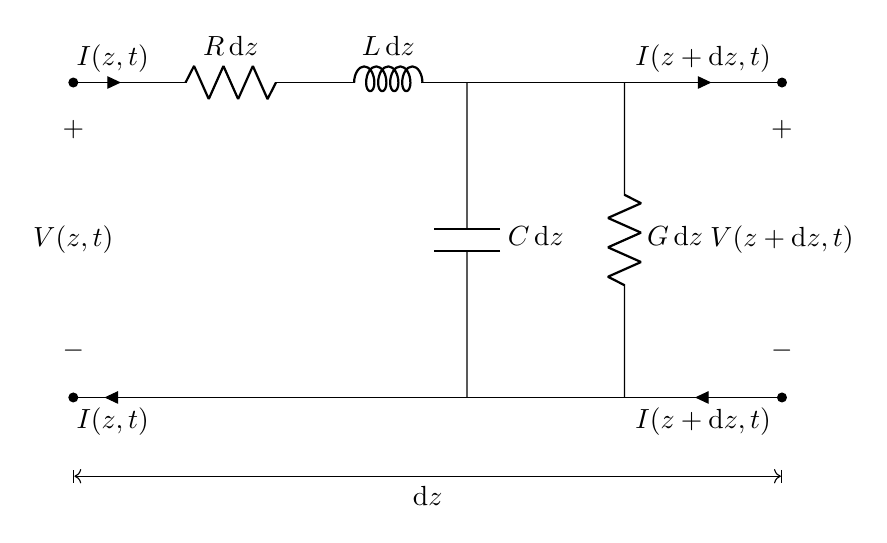
\begin{tikzpicture}
			\draw (0,4) to [short, i = ${I(z,t)}$] (1,4);
			\draw (1,4) to [R = $R \dif z$] (3,4);
			\draw (3,4) to [L = $L \dif z$] (5,4);
			\draw (5,4) to [C = $C \dif z$] (5,0);
			\draw (5,4) to (7,4);
			\draw (7,4) to [R = $G \dif z$] (7,0);
			\draw (7,4) to [short, i = ${I(z + \dif z,t)}$] (9,4);
			\draw (9,0) to [short, i = ${I(z + \dif z,t)}$] (7,0);
			\draw (7,0) to (1,0);
			\draw (1,0) to [short, i = ${I(z,t)}$] (0,0);
			\draw (0,4) to [open, v = ${V(z,t)}$, *-*] (0,0);
			\draw (9,4) to [open, v^= ${V(z + \dif z,t)}$, *-*] (9,0);

			\draw [|<->|] (0,-1) -- (9,-1) node [midway, below] {$\dif z$};
		\end{tikzpicture}
		\caption{Model of Infinitesimal Section of Transmission Line}
		\label{fig:model_of_infinitesimal_section_of_transmission_line}
	\end{figure}
\end{definition}

\section{Telegraph and Wave Equations for a TEM Line}

\begin{theorem}[Telegraph equations]
	For a transmission line directed in the $z$-direction, modelled as in \cref{fig:model_of_infinitesimal_section_of_transmission_line},
	\begin{align*}
		-\dpd{V}{z} &= L \dpd{I}{t} + I R\\
		-\dpd{I}{z} &= C \dpd{V}{t} + G V
	\end{align*}
	\label{thm:telegraph_equations}
\end{theorem}

\begin{proof}
	Let
	\begin{align*}
		V(z + \dif z) - V(z) &= \dif V\\
		I(z + \dif z) - I(z) &= \dif I\\
	\end{align*}
	Therefore,
	\begin{align*}
		\dif V &= -(R \dif z) \left( I(z,t) \right) - (L \dif z) \left( \dod{I(z,t)}{t} \right)\\
		\dif I &= -(C \dif z) \left( \dod{V(z + \dif z,t)}{t} \right) - (G \dif z) \left( V(z + \dif z,t) \right)
	\end{align*}
	Solving,
	\begin{align*}
		-\dpd{V}{z} &= L \dpd{I}{t} + I R\\
		-\dpd{I}{z} &= C \dpd{V}{t} + G V
	\end{align*}
\end{proof}

\begin{definition}[Uniform line]
	A TEM transmission line modelled as in \cref{fig:model_of_infinitesimal_section_of_transmission_line} is said to be uniform if $L$ and $C$ are not functions of $z$.
\end{definition}

\begin{theorem}[Wave equation in a uniform line]
	\begin{align*}
		\left( \dpd[2]{}{z} - L C \dpd[2]{}{t} \right) V(z,t) &= (L G + R C) \dpd{V(z,t)}{t} + R G V V(z,t)\\
		\left( \dpd[2]{}{z} - L C \dpd[2]{}{t} \right) I(z,t) &= (L G + R C) \dpd{I(z,t)}{t} + R G I V(z,t)
	\end{align*}
	\label{thm:wave_equation_in_a_uniform_line}
\end{theorem}

\begin{proof}
	\begin{align*}
		-\dpd{V}{z} &= L \dpd{I}{t} + I R\\
	\end{align*}
	Therefore, differentiating with respect to $z$,
	\begin{align*}
		-\dpd[2]{V}{z} &= L \frac{\partial^2 I}{\partial t \partial z} + R \dpd{I}{z}
	\end{align*}
	Similarly,
	\begin{align*}
		-\dpd{I}{z} &= C \dpd{V}{t} + G V
	\end{align*}
	Therefore, differentiating with respect to $z$,
	\begin{align*}
		-\frac{\partial^2 I}{\partial t \partial z} &= C \dpd[2]{V}{t} + G \dpd{V}{t}
	\end{align*}
	Solving the equations together,
	\begin{align*}
		\left( \dpd[2]{}{z} - L C \dpd[2]{}{t} \right) V(z,t) &= (L G + R C) \dpd{V(z,t)}{t} + R G V V(z,t)\\
		\left( \dpd[2]{}{z} - L C \dpd[2]{}{t} \right) I(z,t) &= (L G + R C) \dpd{I(z,t)}{t} + R G I V(z,t)
	\end{align*}
\end{proof}

\begin{definition}[Power in a line]
	The power in a line along the $z$-direction is
	\begin{align*}
		P(z,t) &= V(z,t) I(z,t)
	\end{align*}
\end{definition}

\begin{theorem}[Poynting Theorem for a General Lossy Line]
	\begin{align*}
		-\dpd{P}{z} &= P_{\text{loss}} + \dpd{}{t}(w_m + w_e)
	\end{align*}
	or equivalently,
	\begin{align*}
		P \Big|_{z_1} - P \Big|_{z_2} &= \int\limits_{z_1}^{z_2} P_{\text{loss}} \dif z + \dpd{}{t} \int\limits_{z_1}^{z_2} (w_m + w_e) \dif z
	\end{align*}
	where
	\begin{align*}
		P_{\text{loss}} &= R I^2 + G V^2
	\end{align*}
	is the power lost over the total resistance,
	\begin{align*}
		w_m &= \frac{1}{2} L I^2
	\end{align*}
	is the magnetic energy stored in the inductor,
	\begin{align*}
		w_e &= \frac{1}{2} C V^2
	\end{align*}
	is the electric energy stored in the capacitor.
	\label{thm:Poynting_theorem_for_a_general_lossy_line}
\end{theorem}

\begin{proof}
	\begin{align*}
		-\dpd{P}{z} &= -\dpd{V I}{z}\\
		&= -\dpd{V}{z} I - \dpd{I}{z} V\\
		&= \left( R I + L \dpd{I}{t} \right) (I) + \left( G V + C \dpd{V}{t} \right) (V)\\
		&= R I^2 + G V^2 + \dpd{}{t}\left( \frac{1}{2} L I^2 + \frac{1}{2} C V^2 \right)
	\end{align*}
\end{proof}

\section{Propagating Waves in Lossless Non-dispersive Transmission Lines}

\begin{definition}[Lossless line]
	A TEM transmission line modelled as in \cref{fig:model_of_infinitesimal_section_of_transmission_line} is said to be lossless if $R$ and $G$ are zero.
\end{definition}

\begin{definition}[Non-dispersive line]
	A TEM transmission line modelled as in \cref{fig:model_of_infinitesimal_section_of_transmission_line} is said to be non-dispersive if $L$ and $C$ are not functions of the frequency.
\end{definition}

\begin{theorem}[Wave equations for lossless, non-dispersive, uniform lines]
	The wave equations for a lossless, non-dispersive, uniform line is
	\begin{align*}
		\left( \dpd[2]{}{z} - L C \dpd[2]{}{t} \right) V(z,t) &= 0\\
		\left( \dpd[2]{}{z} - L C \dpd[2]{}{t} \right) I(z,t) &= 0
	\end{align*}
	\label{thm:wave_equations_for_lossless_non-dispersive_uniform_lines}
\end{theorem}

\begin{definition}[Wavespeed]
	For wave equations as in \cref{thm:wave_equations_for_lossless_non-dispersive_uniform_lines},
	\begin{align*}
		v &= \frac{1}{\sqrt{L C}}
	\end{align*}
	is called the wavespeed.
\end{definition}

\begin{theorem}
	The solutions to the wave equations from \cref{thm:wave_equations_for_lossless_non-dispersive_uniform_lines} are
	\begin{align*}
		V(z,t) &= V^+\left( t - \frac{z}{v} \right) + V^-\left( t + \frac{z}{v} \right) + V_0
	\end{align*}
	and
	\begin{align*}
		I(z,t) &= Y_C \left( V^+\left( t - \frac{z}{v} \right) + V^-\left( t + \frac{z}{v} \right) \right) + I_0
	\end{align*}
	where $V^+$ and $V^-$ are real functions of $t$ which describe the waveforms of the forward and backward propagating waves, respectively, at $z = 0$, $V_0$ and $I_0$ are arbitrary real constants, and $Y_C$ is the characteristic admittance.
	\footnote{See \cref{def:characteristic_impedance}.}
\end{theorem}

\begin{definition}[Characteristic impedance]
	The effective impedance $Z_C$, due to an infinitely long line, i.e. the ratio between the voltage applied to an infinitely long line and the current drawn by it, is called the characteristic impedance of the line.
	Hence,
	\begin{align*}
		Z_C &= \frac{\left| V^+ \right|}{\left| I^+ \right|}\\
		&= \frac{\left| V^- \right|}{\left| I^- \right|}
	\end{align*}
	\label{def:characteristic_impedance}
\end{definition}

\begin{theorem}
	The characteristic impedance for a lossy, non-dispersive, uniform line is
	\begin{align*}
		Z_C &= \sqrt{\frac{L}{C}}
	\end{align*}
	Equivalently, the characteristic admittance is
	\begin{align*}
		Y_C &= \frac{1}{Z_C}\\
		&= \sqrt{\frac{C}{L}}
	\end{align*}
\end{theorem}

\begin{theorem}
	\begin{align*}
		\frac{V}{I} &= Z_C \frac{V^+\left( t - \frac{z}{v} \right) + V^-\left( t + \frac{z}{v} \right)}{V^+\left( t - \frac{z}{v} \right) - V^-\left( t + \frac{z}{v} \right)}
	\end{align*}
\end{theorem}

\clearpage
\part{Circuit Theory of Transmission Lines}

\section{Excitation by Sources}

\begin{theorem}
	An infinite transmission line along the $z$-direction connected as
	\begin{figure}[H]
		\centering
		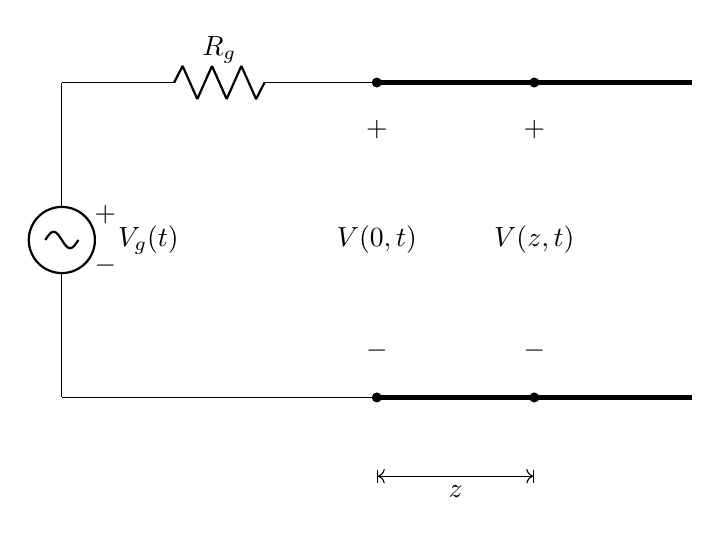
\begin{tikzpicture}
			\draw (0,4) to [sV = ${V_g(t)}$] (0,0);
			\draw (0,4) to [R = $R_g$] (4,4);
			\draw (4,0) to (0,0);
			\draw [ultra thick] (4,4) to (8,4);
			\draw [ultra thick] (4,0) to (8,0);
			\draw [|<->|] (4,-1) -- (6,-1) node [midway, below] {$z$};
			\draw (4,4) to [open, *-*, v = ${V(0,t)}$] (4,0);
			\draw (6,4) to [open, *-*, v^= ${V(z,t)}$] (6,0);
		\end{tikzpicture}
	\end{figure}
	is equivalent to
	\begin{figure}[H]
		\centering
		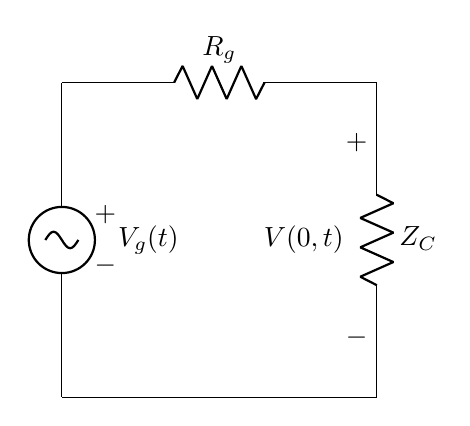
\begin{tikzpicture}
			\draw (0,4) to [sV = ${V_g(t)}$] (0,0);
			\draw (0,4) to [R = $R_g$] (4,4);
			\draw (4,4) to [R = $Z_C$, v = ${V(0,t)}$] (4,0);
			\draw (4,0) to (0,0);
		\end{tikzpicture}
	\end{figure}
	and hence
	\begin{align*}
		V(z,t) &= \frac{Z_C}{R_g + Z_C} V_g \left( t - \frac{z}{v} \right)\\
		I(z,t) &= \frac{1}{R_g + Z_C} V_g \left( t - \frac{z}{v} \right)
	\end{align*}
\end{theorem}

\begin{question}
	An infinite transmission line is connected to a voltage source
	\begin{align*}
		S(t) &= e^{-\alpha t} u(t)
	\end{align*}
	as shown.
	\begin{figure}[H]
		\centering
		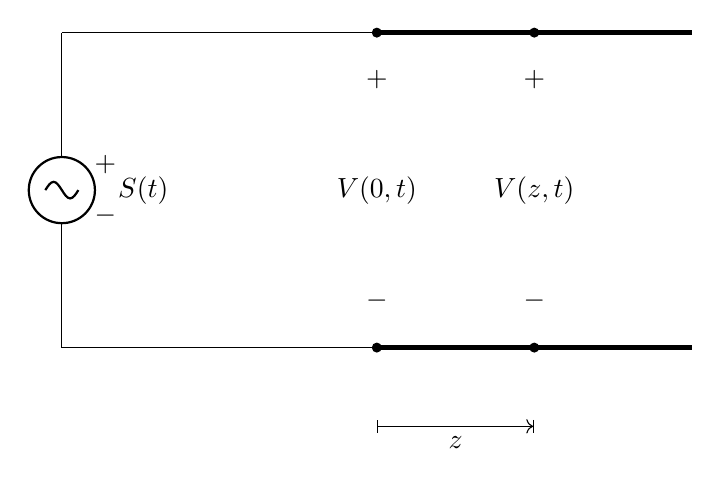
\begin{tikzpicture}
			\draw (0,4) to [sV = ${S(t)}$] (0,0);
			\draw (0,4) to (4,4);
			\draw (4,0) to (0,0);
			\draw [ultra thick] (4,4) to (8,4);
			\draw [ultra thick] (4,0) to (8,0);
			\draw [|->|] (4,-1) -- (6,-1) node [midway, below] {$z$};
			\draw (4,4) to [open, *-*, v = ${V(0,t)}$] (4,0);
			\draw (6,4) to [open, *-*, v^= ${V(z,t)}$] (6,0);
		\end{tikzpicture}
	\end{figure}
	\begin{enumerate}
		\item Find $V(z,t)$.
		\item Find $I(z,t)$.
		\item Plot $V(z,t)$ for $\alpha = 1$.
	\end{enumerate}
\end{question}

\begin{solution}
	\begin{enumerate}
		\item
			\begin{align*}
				V(z,t) &= V^+\left( t - \frac{z}{v} \right) + V^-\left( t + \frac{z}{v} \right) + V_0
			\end{align*}
			Assuming $V_0$ to be zero, and as the wire is infinite assuming $V^-$ to be a constant zero,
			\begin{align*}
				V(z,t) &= V^+\left( t - \frac{z}{v} \right)
			\end{align*}
			Therefore,
			\begin{align*}
				V^+(t) &= V(0,t)\\
				&= S(t)
			\end{align*}
			Hence,
			\begin{align*}
				V(z,t) &= V^+\left( t - \frac{z}{v} \right)\\
				&= S\left( t - \frac{z}{v} \right)\\
				&= e^{-\alpha \left( t - \frac{z}{v} \right)} u\left( t - \frac{z}{v} \right)
			\end{align*}
		\item
			As for $V(z,t)$,
			\begin{align*}
				I(z,t) &= I^+\left( t - \frac{z}{v} \right)\\
				&= Y_C V^+\left( t - \frac{z}{v} \right)\\
				&= Y_C e^{-\alpha \left( t - \frac{z}{v} \right)} u\left( t - \frac{z}{v} \right)
			\end{align*}
		\item
			The forward propagating wave has behaviour of the form
			\begin{figure}[H]
				\centering
				\begin{tikzpicture}
					\def\xMIN{0};
					\def\xMAX{5};
					\def\yMIN{0};
					\def\yMAX{5};

					\begin{scope}[-stealth]
						\draw (\xMIN,0) -- (\xMAX,0) node [right] {$t$};
						\draw (0,\yMIN) -- (0,\yMAX) node [above] {$V^+(t,z_0)$};
					\end{scope}

					\begin{scope}
						\draw (0,0) -- (1,0) -- (1,3) to [out = -90, in = 180] (3,0);
					\end{scope}
				\end{tikzpicture}
			\end{figure}
			\begin{figure}[H]
				\centering
				\begin{tikzpicture}
					\def\xMIN{0};
					\def\xMAX{5};
					\def\yMIN{0};
					\def\yMAX{5};

					\begin{scope}[-stealth]
						\draw (\xMIN,0) -- (\xMAX,0) node [right] {$z$};
						\draw (0,\yMIN) -- (0,\yMAX) node [above] {$V^+(t_0,z)$};
					\end{scope}

					\begin{scope}
						\draw (0,0) to [out = 0, in = -90] (3,3) -- (3,0) -- (4,0);
					\end{scope}
				\end{tikzpicture}
			\end{figure}
	\end{enumerate}
\end{solution}

\section{Reflections at Loads}

\begin{definition}[Reflection coefficient]
	The reflection coefficient at a junction is defined to be
	\begin{align*}
		\Gamma &= \frac{V^-(t)}{V^+(t)}
	\end{align*}
	where $V^+(t)$ is the incident wave and $V^-(t)$ is the reflected wave.
\end{definition}

\begin{definition}[Transmission coefficient]
	The reflection coefficient at a junction is defined to be
	\begin{align*}
		\tau &= \frac{{V_2}^+(t)}{{V_1}^+(t)}
	\end{align*}
	where ${V_1}^+(t)$ is the incident wave and ${V_2}^+(t)$ is the transmitted wave.
\end{definition}

\begin{theorem}
	For a forward propagating wave $V^+(z,t)$ propagating over an infinite transmission line, with characteristic impedance $Z_C$, extending from $z \to -\infty$ to $z = 0$, terminated at $z = 0$ by a load with resistance $R_L$, the reflection coefficient is
	\begin{align*}
		\Gamma_L &= \frac{R_L - Z_C}{R_L + Z_C}
	\end{align*}
	and hence
	\begin{align*}
		V(z,t) &= V^+\left( t - \frac{z}{v} \right) + \frac{R_L - Z_C}{R_L + Z_C} V^+\left( t + \frac{z}{v} \right)\\
		I(z,t) &= Y_C \left( V^+\left( t - \frac{z}{v} \right) - \frac{R_L - Z_C}{R_L + Z_C} V^+\left( t + \frac{z}{v} \right) \right)
	\end{align*}
\end{theorem}

\begin{solution}
	For $z < 0$,
	\begin{align*}
		V(z,t) &= V^+\left( t - \frac{z}{v} \right) + V^-\left( t + \frac{z}{v} \right)\\
		I(z,t) &= Y_C V^+\left( t - \frac{z}{v} \right) + Y_C V^-\left( t + \frac{z}{v} \right)
	\end{align*}
	By Ohm's Law,
	\begin{align*}
		\frac{V_L}{I_L} &= R_L
	\end{align*}
	where $V_L$ and $I_L$ are the voltage across and current through the load.
	Therefore,
	\begin{align*}
		V_L &= V(0,t)\\
		&= V^+(t) + V^-(t)\\
		I_L &= V(0,t)\\
		&= Y_C \left( V^+(t) - V^-(t) \right)
	\end{align*}
	Therefore,
	\begin{align*}
		R_L &= \frac{V^+(t) + V^-(t)}{Y_C\left( V^+(t) - V^-(t) \right)}\\
		\therefore V^-(t) &= V^+(t) \frac{R_L - Z_C}{R_L + Z_C}
	\end{align*}
	Therefore, the reflection coefficient is
	\begin{align*}
		\Gamma_L &= \frac{R_L - Z_C}{R_L + Z_C}
	\end{align*}
	Hence,
	\begin{align*}
		V(z,t) &= V^+\left( t - \frac{z}{v} \right) + V^-\left( t + \frac{z}{v} \right)\\
		&= V^+\left( t - \frac{z}{v} \right) + \Gamma_L V^+\left( t + \frac{z}{v} \right)\\
		&= V^+\left( t - \frac{z}{v} \right) + \frac{R_L - Z_C}{R_L + Z_C} V^+\left( t + \frac{z}{v} \right)\\
		I(z,t) &= Y_C V^+\left( t - \frac{z}{v} \right) + Y_C V^-\left( t + \frac{z}{v} \right)\\
		&= Y_C \left( V^+\left( t - \frac{z}{v} \right) - \Gamma_L V^+\left( t + \frac{z}{v} \right) \right)\\
		&= Y_C \left( V^+\left( t - \frac{z}{v} \right) - \frac{R_L - Z_C}{R_L + Z_C} V^+\left( t + \frac{z}{v} \right) \right)
	\end{align*}
\end{solution}

\section{Reflection and Transmission at Discontinuities}

\begin{theorem}
	A system of two infinite transmission lines, with characteristic impedances ${Z_C}_1$ and ${Z_C}_2$ and wave propagation speeds $v_1$ and $v_2$, connected as
	\begin{figure}[H]
		\centering
		\begin{tikzpicture}
			\draw [ultra thick] (0.2,4) to (4,4);
			\draw [ultra thick] (0.2,0) to (4,0);
			\draw [ultra thick] (-0.2,4) to (-4,4);
			\draw [ultra thick] (-0.2,0) to (-4,0);
			\draw (-0.2,0) to (0.2,0);
			\draw (-0.2,4) to (0.2,4);
			\draw [dashed] (0,-1) to (0,5) node [above] {$z = 0$};

			\draw (-2,4) to [open, *-*, v^= ${V_1(z,t)}$] (-2,0);
			\draw (2,4) to [open, *-*, v^= ${V_2(z,t)}$] (2,0);
		\end{tikzpicture}
	\end{figure}
	is equivalent to
	\begin{figure}[H]
		\centering
		\begin{tikzpicture}
			\draw [ultra thick] (-0.2,4) to (-4,4);
			\draw [ultra thick] (-0.2,0) to (-4,0);
			\draw (-0.2,4) to (1,4);
			\draw (-0.2,0) to (1,0);
			\draw (1,0) to [R = ${Z_C}_2$] (1,4);
			\draw [dashed] (0,-1) to (0,5) node [above] {$z = 0$};

			\draw (-2,4) to [open, *-*, v^= ${V_1(z,t)}$] (-2,0);
		\end{tikzpicture}
	\end{figure}
	and hence
	\begin{align*}
		\Gamma &= \frac{{Z_C}_2 - {Z_C}_1}{{Z_C}_2 + {Z_C}_1}\\
		\tau &= \frac{2 {Z_C}_2}{{Z_C}_2 + {Z_C}_1}
	\end{align*}
\end{theorem}

\begin{proof}
	Let the waves propagating in the lines be ${V_1}^+$, ${V_1}^-$, and ${V_2}^+$.
	\footnote{The second line is infinite in the positive direction, and is excited by the first line only. Hence, there is no backward propagating wave ${V_2}^-$.}
	\begin{align*}
		V_1(z,t) &= {V_1}^+\left( t - \frac{z}{v_1} \right) + {V_1}^-\left( t + \frac{z}{v_1} \right)\\
		\therefore I_1(z,t) &= {Y_C}_1 {V_1}^+\left( t - \frac{z}{v_1} \right) - {V_1}^-\left( t + \frac{z}{v_1} \right)\\
		V_2(z,t) &= {V_2}^+\left( t - \frac{z}{v_1} \right)\\
		\therefore I_2(z,t) &= {Y_C}_2 {V_1}^+\left( t - \frac{z}{v_1} \right)
	\end{align*}
	Therefore, as the voltage and current are continuous at $z = 0$,
	\begin{align*}
		{V_1}^+(t) (1 + \Gamma) &= {V_1}^+(t) \tau\\
		{Y_C}_1 {V_1}^+(t) (1 - \Gamma) &= {Y_C}_2 {V_1}^+(t) \tau
	\end{align*}
	Therefore,
	\begin{align*}
		1 + \Gamma &= \tau\\
		{Y_C}_1 (1 - \Gamma) &= {Y_C}_2 \tau
	\end{align*}
	Therefore,
	\begin{align*}
		\Gamma &= \frac{{V_1}^-(t)}{{V_1}^+(t)}\\
		&= \frac{{Z_C}_2 - {Z_C}_1}{{Z_C}_2 + {Z_C}_1}\\
		\tau &= \frac{2 {Z_C}_2}{{Z_C}_2 + {Z_C}_1}
	\end{align*}
	Therefore, the second line is equivalent to a load with impedance ${Z_C}_2$.
\end{proof}

\section{Reflection and Transmission at Junction with Composite Load}

\begin{theorem}
	A system of two infinite transmission lines, with characteristic impedances ${Z_C}_1$ and ${Z_C}_2$ and wave propagation speeds $v_1$ and $v_2$, and a lumped resistance, connected as
	\begin{figure}[H]
		\centering
		\begin{tikzpicture}
			\draw [ultra thick] (0.2,4) to (4,4);
			\draw [ultra thick] (0.2,0) to (4,0);
			\draw [ultra thick] (-0.2,4) to (-4,4);
			\draw [ultra thick] (-0.2,0) to (-4,0);
			\draw (-0.2,0) to (0.2,0);
			\draw (-0.2,4) to (0.2,4);
			\draw (0,0) to [R = $R$] (0,4);
			\draw [dashed] (0,-1) to (0,5) node [above] {$z = 0$};

			\draw (-2,4) to [open, *-*, v^= ${V_1(z,t)}$] (-2,0);
			\draw (2,4) to [open, *-*, v^= ${V_2(z,t)}$] (2,0);
		\end{tikzpicture}
	\end{figure}
	is equivalent to
	\begin{figure}[H]
		\centering
		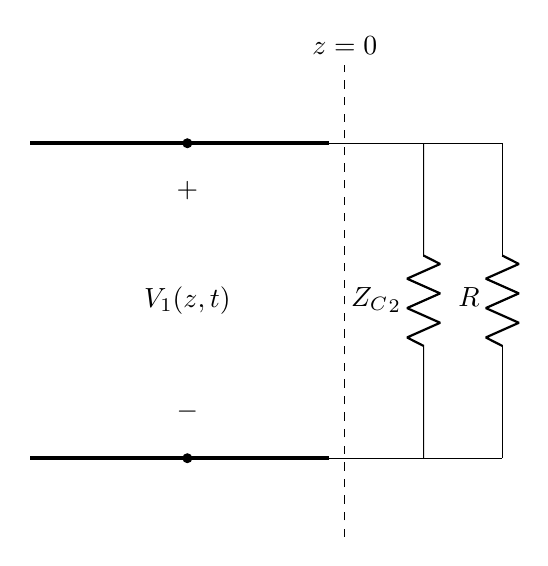
\begin{tikzpicture}
			\draw [ultra thick] (-0.2,4) to (-4,4);
			\draw [ultra thick] (-0.2,0) to (-4,0);
			\draw (-0.2,4) to (2,4);
			\draw (-0.2,0) to (2,0);
			\draw (1,0) to [R = ${Z_C}_2$] (1,4);
			\draw (2,0) to [R = $R$] (2,4);
			\draw [dashed] (0,-1) to (0,5) node [above] {$z = 0$};

			\draw (-2,4) to [open, *-*, v^= ${V_1(z,t)}$] (-2,0);
		\end{tikzpicture}
	\end{figure}
	and hence
	\begin{align*}
		\Gamma &= \frac{({Z_C}_2 \parallel R) - {Z_C}_1}{({Z_C}_2 \parallel R) + {Z_C}_1}\\
		\tau &= \frac{2 ({Z_C}_2 \parallel R)}{({Z_C}_2 \parallel R) + {Z_C}_1}
	\end{align*}
\end{theorem}

\section{Reverberations in Transmission Lines}

\begin{theorem}
	The voltage and current in a line with $Z_C$ and $v$ excited at $z = 0$ by a source $V_g(t)$ with internal impedance $R_g$ and terminated by a resistive load $R_L$ at $z = l$ are
	\begin{align*}
		V(z,t) &= V_0 + \sum\limits_{n = 1}^{\infty} {V_n}^+\left( t - \frac{z}{v} \right) + {V_n}^-\left( t + \frac{z}{v} \right)\\
		&= \frac{Z_C}{R_g + Z_C} \left( V_g\left( t - \frac{z}{v} \right) + \Gamma_L V_g\left( t - 2 T + \frac{z}{v} \right) + \Gamma_L \Gamma_g V_g\left( t - 3 T - \frac{z}{v} \right) + \dots \right)\\
		I(z,t) &= I_0 + Y_C \sum\limits_{n = 1}^{\infty} {V_n}^+\left( t - \frac{z}{v} \right) - {V_n}^-\left( t + \frac{z}{v} \right)\\
		&= \frac{1}{R_g + Z_C} \left( V_g\left( t - \frac{z}{v} \right) + \Gamma_L V_g\left( t - 2 T + \frac{z}{v} \right) + \Gamma_L \Gamma_G V_g\left( t - 3 T - \frac{z}{v} \right) + \dots \right)
	\end{align*}
	where $\Gamma_L$ and $\Gamma_G$ are the reflection coefficients at the load junction and the source junction respectively.
\end{theorem}

\begin{theorem}
	The voltage and current in a line with $Z_C$ and $v$ excited at $z = 0$ by a step input of height ${V_g}_0$ with internal impedance $R_g$ and terminated by a resistive load $R_L$ at $z = l$ are
	\begin{align*}
		V(z,t) &= {V_g}_0 \frac{Z_C}{R_g + Z_C} (1 + \Gamma_L) \sum\limits_{n = 0}^{\infty} (\Gamma_L \Gamma_g)^n\\
		&= {V_g}_0 \frac{R_L}{R_g + R_L}\\
		V(z,t) &= {V_g}_0 \frac{1}{R_g + Z_C} (1 - \Gamma_L) \sum\limits_{n = 0}^{\infty} (\Gamma_L \Gamma_g)^n\\
		I(z,t) &= {V_g}_0 \frac{1}{R_g + R_L}
	\end{align*}
\end{theorem}

\end{document}
